\begin{enumerate}[label=\thesubsection.\arabic*.,ref=\thesubsection.\theenumi]
\numberwithin{equation}{enumi}
\numberwithin{figure}{enumi}


\item   Fig. \ref{fig:ee18btech11025} shows  the Bode magnitude and phase plots of 
    \begin{equation}  
            G(s) = \frac{n_0}{s^3 + d_2 s^2 + d_1 s + d}
    \end{equation}
\begin{figure}[ht!]
        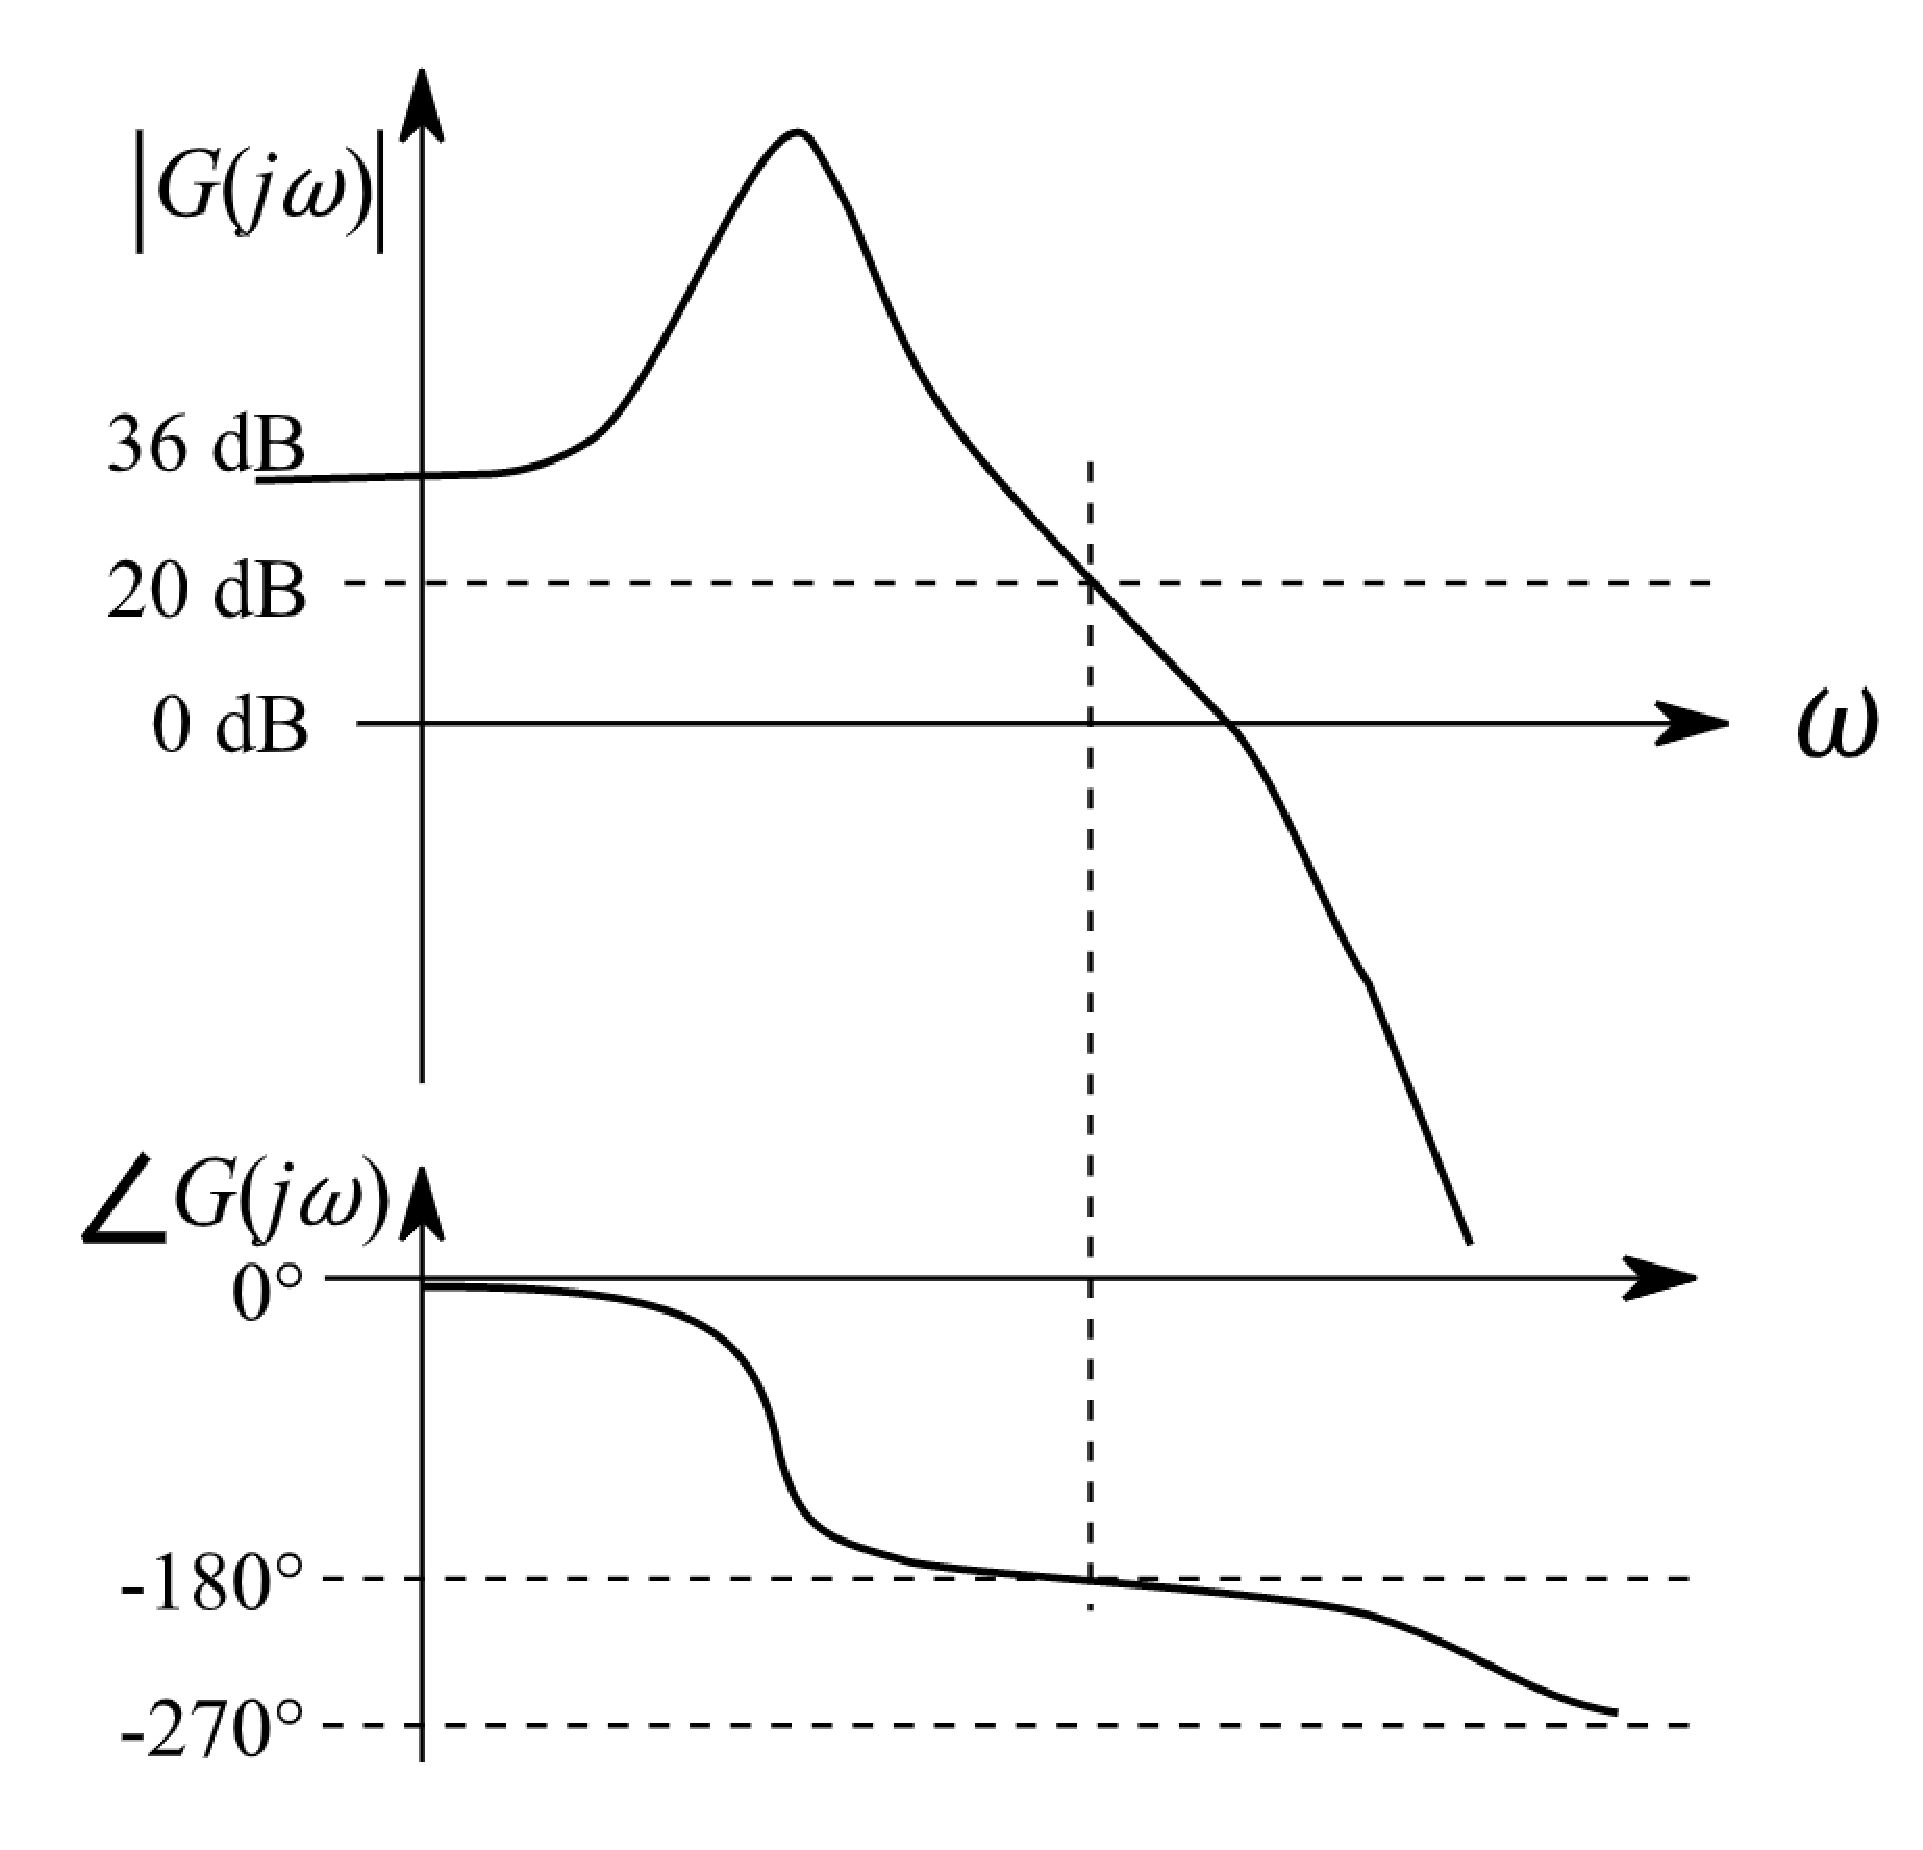
\includegraphics[width=\columnwidth]{./figs/ee18btech11025/q42_1.eps}
        \caption{}
        \label{fig:ee18btech11025}
\end{figure}
Find  $\abs{G\brak{\j\omega_{pc}}}$.
\\
\solution From Fig. \ref{fig:ee18btech11025}, 
%
\begin{align}
\angle G\brak{\j\omega_{pc}}  &= 180 \degree
\\
\implies 20\log\abs{ G\brak{\j\omega_{pc}}}  &= 20
\label{ee18btech11025_g_gain}
%
\end{align}
%


\item  Consider the negative unity feedback configuration with gain $k$ in the feed forward path as shown in Fig.     \ref{fig:ee18btech11025_bock}.  Find the condition for the closed loop system to be stable.
%
\begin{figure}[!ht]
	\begin{center}
		
		\resizebox{\columnwidth}{!}{\begin{enumerate}[label=\thesection.\arabic*.,ref=\thesection.\theenumi]
1. The figure below shows the Bode magnitude and phase plots of a stable transfer function:
\begin{equation}  
            G(s) = \frac{n_0}{s^3 + d_2 s^2 + d_1 s + d}
\end{equation}
 
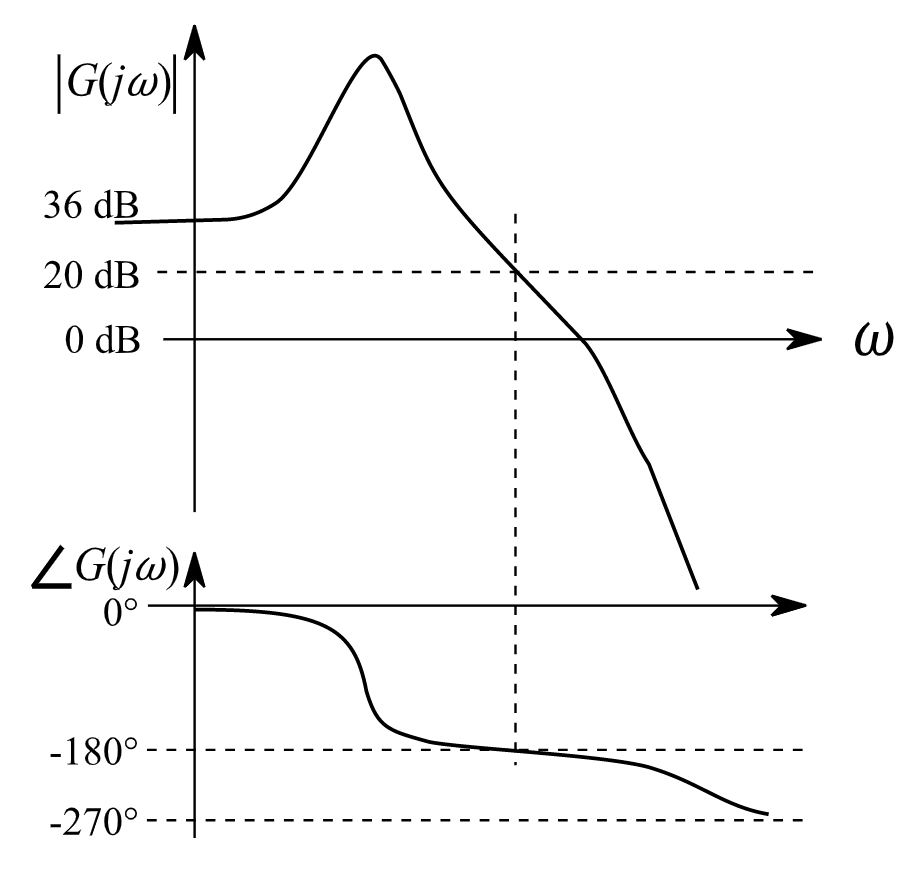
\includegraphics[scale = 0.25]{q42 (1).png}
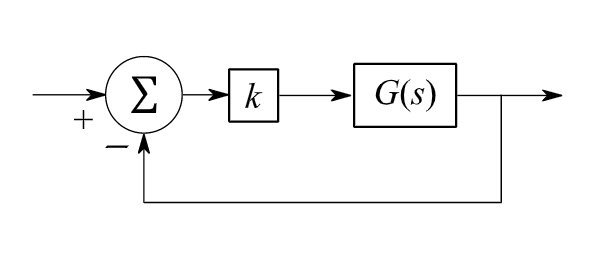
\includegraphics[scale = 0.4]{q42.png}
 Consider the negative unity feedback configuration with gain $k$ in the feed forward path. The closed loop is stable for  . 
    The maximum value of $k_o$  is: \\


\textbf{ Solution:}

\begin{align}   

\begin{equation}
   \\ K_g = \frac{1}{|G(j\omega)|}
\end{equation} 
$K_g$ is the gain margin
at the frequency at which phase angle
is -180\degree.
\\\\ 
In terms of decibels: 
 \begin{equation}
    K_g dB = -20log(|G(j\omega)|) dB
\end{equation}


1.For a stable system, Gain margin at the phase cross-over frequency \textgreater \ 0dB. \\
2.The phase crossover frequency is the frequency at which the phase angle first reaches -180\degree. \\
3.The gain margin refers to the amount of gain, which can be increased or decreased without making the system unstable. \\
4.Gain margin is the factor by which the gain must be multiplied at the phase crossover to have the value 1. \\
5.The phase crossover frequency is the frequency at which the phase angle first reaches -180\degree and thus is the point where the Nyquist plot crosses the real axis. \\

    

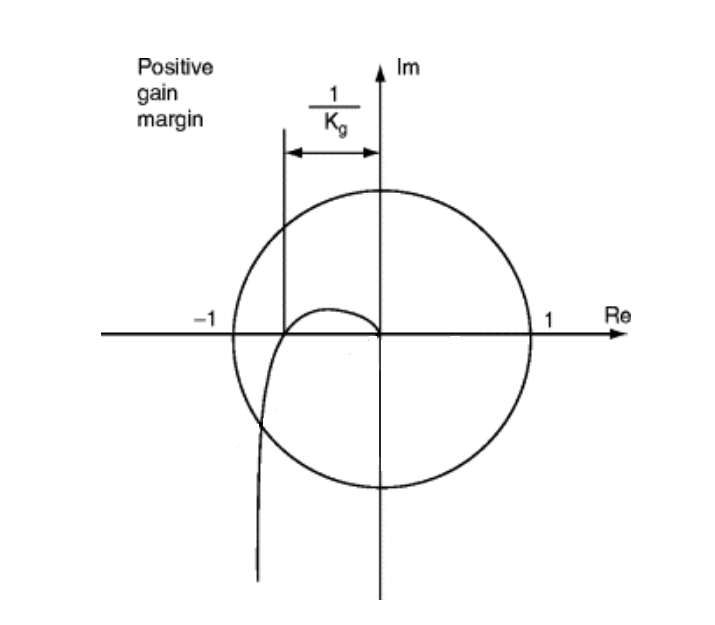
\includegraphics[scale = 0.52]{1.png}
Fig: nyquist plot of stable transfer function 

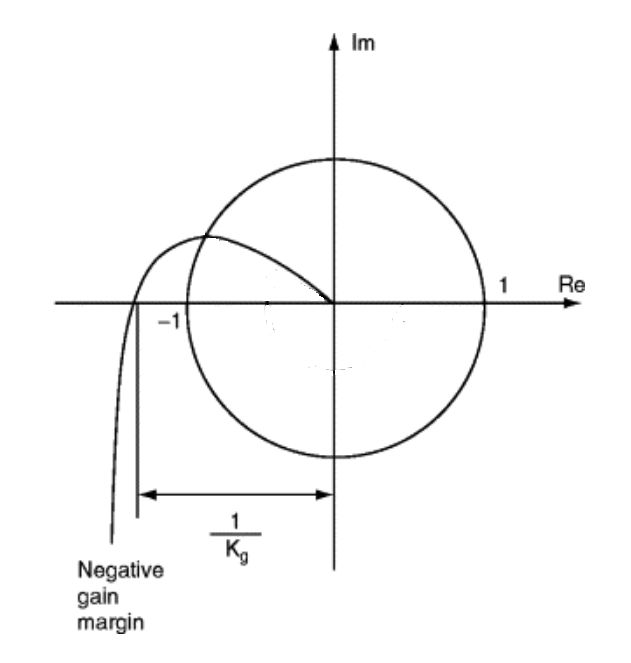
\includegraphics[scale = 0.33]{2.png} 
 \\ Fig: nyquist plot of unstable transfer function
\\
\\ For a stable system, Gain margin at the phase \ \ cross-over frequency \textgreater \ 1.
\\
\\ G(s) is cascaded with k, so,
\begin{equation}
        G_1(s) = kG(s) \\
        \centering
\end{equation}
\begin{equation}
        K_g = \frac{1}{|G_1(j\omega_p_c)|} \textgreater 1\\
        \centering
\end{equation}
\begin{equation}
\implies K_g_(_d_B_) = -20log(|G_1(j\omega_p_c)|) \textgreater \ 0dB
    
\end{equation}

\begin{equation}
    \implies  -20log(|G(j\omega_p_c)k|) \textgreater \ 0dB
    \centering
\end{equation}

\begin{equation}
    \implies  -20 - 20log(|k|) \textgreater \ 0dB
    \centering
\end{equation}

\begin{equation}
   \implies 20log(k) \ \textless \ -20
   \centering
\end{equation}

\begin{equation}
    \implies k \ \textless \ 10^-^1
\end{equation}

\begin{equation}
    \implies k_m_a_x = 0.1
    \centering
\end{equation}

\therefore \ $k_o$ = 0.1

\end{align}
\end{enumerate}
}
	\end{center}
\caption{}
    \label{fig:ee18btech11025_bock}
\end{figure}
\\
\solution The open loop gain for the system in    Fig.  \ref{fig:ee18btech11025_bock} is
%
    \begin{align}  
            G_1(s) &= kG(s)
\\
\implies \angle G_1\brak{\j\omega_{pc}}  &= \angle G\brak{\j\omega_{pc}}  
\\
&= 180 \degree \quad \text{and}
\\
 20\log\abs{ G_1\brak{\j\omega_{pc}}}  &= 20\log \abs{k }+20\log\abs{ G\brak{\j\omega_{pc}}}
\\
&= 20 \brak{1 + \log \abs{k }}
\label{ee18btech11025_g1_gain}
    \end{align}
from \eqref{ee18btech11025_g_gain}.  From \eqref{eq:ee18btech11016_gm_def} and \eqref{ee18btech11025_g1_gain}, the GM of $G_1(s)$ is
    \begin{align}  
-20\log \abs{ G_1\brak{\j\omega_{pc}}} &= -20 \brak{1 + \log \abs{k }}
    \end{align}
%
For stability, $GM > 0$
    \begin{align}  
\implies  -20 \brak{1 + \log \abs{k }} &> 0
\\
\implies  \abs{k} &< 0.1
    \end{align}
%
\end{enumerate}

